\section{Лекция №13 (11.12.2023)}

\textit{Отменена, далее~--- высланный конспект. Судя по всему, это скан с пособия Г.~А.~Доррера <<Методы моделирования дискретных систем>>, 2004 г.}

\begin{dd}
    Сеть Петри~--- это математическая модель дискретных динамических систем (параллельных программ, операционных систем, ЭВМ и их устройств, сетей ЭВМ), ориентированная на качественный анализ и синтез таких систем (обнаружение блокировок, тупиковых ситуаций и узких мест, автоматический синтез параллельных программ и компонентов ЭВМ и др.).
\end{dd}

Формально в терминах теории систем сеть Петри (Petri Net~--- PN)~--- это набор элементов (кортеж):
%
\begin{equation*}
    \text{PN} = \{ \Theta, P, T, F, M_0 \}
\end{equation*}
%
Здесь:

\begin{enumerate}
    \item ${\Theta = \{ 0, 1, 2, \dots \}}$~--- множество дискретных моментов времени.
    \item ${P = \{ p_1, p_2, \dots, p_n \}}$~--- непустое множество элементов сети, называемых \textit{позициями} (местами).
    \item ${T = \{ t_1, t_2, \dots, t_m \}}$~--- непустое множество элементов сети, называемых \textit{переходами}.
    
    Множества позиций и переходов не пересекаются: ${ P\cap T = \varnothing }$.

    \item ${F\colon (P\times T)\cup(T\times P)\rightarrow \{ 0, 1, 2, \dots, k, \dots \}}$~--- функция инцидентности, где $k$~--- кратность дуги.
    \item ${M_0\colon P\rightarrow \{ 0, 1, 2, \dots \}}$~--- начальная маркировка позиций.
\end{enumerate}

Функция инцидентности может быть представлена в виде ${F = F^p\cup F^t}$ и фактически задает два отображения:

\begin{itemize}
    \item ${F^p(p, t) = P\times T\rightarrow \{ 0, 1, 2, \dots \}}$, то есть для каждой позиции указываются связанные с ней переходы (с учетом их кратности);
    \item ${F^t(t, p) = T\times P\rightarrow \{ 0, 1, 2, \dots \}}$, то есть для каждого перехода указываются связанные с ним позиции (также с учетом кратности).
\end{itemize}

Эти функции, в общем случае зависящие от времени, могут быть представлены \textit{матрицами инцидентности}:
%
\begin{equation*}
    \renewcommand*{\arraystretch}{1.75}
    F^p = \begin{blockarray}{ccccc}
        t_1 & t_2 & \cdots & t_m & \\
        \begin{block}{[cccc]c}
          f_{11}^p & f_{12}^p & \cdots & f_{1m}^p & p_1\\
          \vdots & \vdots & \vdots & \vdots & \vdots\\
          f_{n1}^p & f_{n2}^p & \cdots & f_{nm}^p & p_n\\
        \end{block}
        \end{blockarray}
        \quad\quad
    F^t = \begin{blockarray}{ccccc}
        p_1 & p_2 & \cdots & p_n & \\
        \begin{block}{[cccc]c}
          f_{11}^t & f_{12}^t & \cdots & f_{1n}^t & t_1\\
          \vdots & \vdots & \vdots & \vdots & \vdots\\
          f_{m1}^t & f_{m2}^t & \cdots & f_{mn}^t & t_m\\
        \end{block}
        \end{blockarray}
\end{equation*}
%
Из вершины-позиции ${p_i\in P}$ ведет дуга в вершину-переход ${t_j\in T}$ тогда и только тогда, когда ${f_{ij}^p > 0}$. В этом случае говорят, что $t_j$~--- выходной переход позиции $p_i$.

Множество всех позиций $p_k$, для которых $t_j$~--- выходной переход, будем обозначать $P^j$. Иными словами, ${P^j = \{p_k\colon f_{kj}^p > 0 \}}$.

Аналогично из каждой вершины перехода ${t_j\in T}$ дуга ведет в вершину-позицию ${p_i\in P}$ тогда и только тогда, когда ${f_{ji}^t > 0}$. При этом говорят, что $p_i$~--- выходная позиция перехода $t_j$. 

Множество всех переходов $t_l$, для которых $p_i$~--- выходная позиция, будем обозначать $T^i$. Таким образом, ${T^i = \{ t_l\colon f_{li}^t > 0 \}}$. При ${f_{ij}^p > 0}$ и ${f_{ji}^t > 0}$ эти величины называются \textit{кратностью} соответствующих дуг.

Каждая позиция ${p_i\in P}$ может содержать некоторый целочисленный ресурс ${\mu(p)\geqslant 0}$, часто отображаемый соответствующим числом точек (фишек) внутри позиции~--- рисунок~\ref{img:13/inc/chips}.

Вектор ${M = [\mu_1, \dots, \mu_n]}$ называют \textit{маркировкой (разметкой) сети Петри}. Каждая маркировка~-- это отображение ${M\colon P\rightarrow \{0, 1, 2, \dots \}}$. Начальная маркировка $M_0$ определяет стартовое состояние сети Петри.

Смена маркировок (начиная с $M_0$) происходит в результате срабатывания переходов сети. Переход ${t_j\in T}$ может сработать при маркировке $M$, если для всех ${p_i\in P^j}$ выполняется условие ${\mu_i(\theta) - f_{ij}^p(\theta)\geqslant 0}$, то есть если каждая входная позиция для данного перехода ${p_i\in P^j}$ содержит как минимум столько фишек, какова кратность ведущей к $t_j$ дуги.

В результате срабатывания перехода $t_j$ в момент времени $\theta$ маркировка $M(\theta)$ сменяется маркировкой $M(\theta + 1)$ по правилу~(\ref{eq:rule}):
%
\begin{equation}
    \label{eq:rule}
\begin{gathered}
    \mu_i(\theta + 1) = \mu_i(\theta) - f_{ij}^p(\theta) + f_{ji}^t(\theta)\\
    i = \overline{1, n},\, j = \overline{1, m},\, i\in P^j,\, j\in T^i
\end{gathered}
\end{equation}
%
Иными словами, переход $t$ изымает из каждой своей входной позиции число фишек, равное кратности входных дуг, и посылает в каждую свою выходную позицию число фишек, равное кратности выходных дуг.

Если может сработать несколько переходов, то срабатывает один (любой из них). Функционирование сети останавливается, если при некоторой \textit{тупиковой маркировке} ни один из ее переходов не может сработать. При одной и той же начальной маркировке сеть Петри может порождать, в силу недетерминированности ее функционирования, различные последовательности срабатывания ее переходов. Эти последовательности образуют \textit{слова} в алфавите $T$.

Множество всевозможных слов, порождаемых сетью Петри, называют \textit{языком} сети Петри. Две сети Петри эквивалентны, если они порождают один и тот же язык.

В отличие от конечных автоматов, в терминах которых описываются глобальные состояния систем, сети Петри концентрируют внимание на локальных событиях (переходах), локальных условиях (позициях) и локальных связях между событиями и условиями. Поэтому в терминах сетей Петри более адекватно, чем с помощью автоматов, моделируется поведение распределенных асинхронных систем.

\subsection{Графы сетей Петри}

Формальное определение сети Петри, изложенное выше, полностью определяет ее функционирование. Однако при решении конкретных инженерных задач удобнее и нагляднее графическое представление этих сетей. 

Теоретико-графовым представлением сети Петри является двудольный ориентированный мультиграф сети Петри, который содержит:

\begin{itemize}
    \item позиции (места), обозначаемые кружками;
    \item переходы, обозначаемые планками;
    \item ориентированные дуги (стрелки), соединяющие позиции с переходами и переходы с позициями (кратные дуги обозначаются несколькими параллельными дугами).
\end{itemize}

Благодаря наличию кратных дуг сеть Петри есть мультиграф. Благодаря двум типам вершин граф называется двудольным. Поскольку дуги имеют направление, граф является ориентированным. Пример такого мультиграфа показан на рисунке~\ref{img:13/inc/chips}.

\image
{.5\textwidth}
{13/inc/chips}
{Пример графа сети Петри}

Для сети, изображенной на этом рисунке, матрицы инцидентности имеют вид
%
\begin{equation*}
    \renewcommand*{\arraystretch}{1.75}
    F^p = \begin{blockarray}{ccccc}
        t_1 & t_2 & t_3 & t_4 & \\
        \begin{block}{[cccc]c}
          1 & 1 & 0 & 0 & p_1\\
          0 & 2 & 0 & 0 & p_2\\
          0 & 0 & 1 & 1 & p_3\\
        \end{block}
        \end{blockarray}
        \quad\quad
    F^t = \begin{blockarray}{cccc}
        p_1 & p_2 & p_3 & \\
        \begin{block}{[ccc]c}
            1 & 1 & 0 & t_1\\
            0 & 0 & 1 & t_2\\
            1 & 2 & 0 & t_3\\
            1 & 0 & 0 & t_4\\
        \end{block}
        \end{blockarray}
\end{equation*}
%
Начальная маркировка, как видно из рисунка,~--- ${M_0 = [2, 2, 0]}$.

Нетрудно видеть, что матричное и графовое представления взаимно однозначно соответствуют друг другу.

В случае большой кратности дуг ее можно указывать цифрами на соответствующей дуге.

\subsection{Пространство состояний сети Петри}

Состояние сети Петри определяется ее маркировкой. Пространство состояний сети Петри, обладающей $n$ позициями, есть множество всех маркировок, то есть $E^n$. 

Изменение в состоянии, вызванное запуском перехода, определяется функцией перехода $\delta$ или функцией следующего состояния. Когда эта функция применяется к маркировке $M$ и переходу $t_j$ (если он разрешен), то в соответствии с~(\ref{eq:rule}) получается новая маркировка ${M' = \delta(M, t_j)}$. Она, как уже говорилось, получается изъятием фишек из позиции $p_i$ таких, что ${f_{ij}^p\neq 0}$ (${\mu_i\geqslant f_{ij}^p}$) и помещением фишек в позиции $p_k$ такие, что ${f_{ik}^t\neq 0}$. 

Процесс создания новых маркировок продолжается до тех пор, пока в сети Петри при данной маркировке существует хоть один разрешенный переход. Если же при некоторой маркировке ни один переход не разрешен, то такая маркировка называется тупиковой.

При выполнении сети Петри получается две последовательности:

\begin{itemize}
    \item последовательность маркировок ${\{ M(0), M(1), M(2), \dots \}}$;
    \item последовательность запущенных переходов ${\{ t_{j0}, t_{j1}, t_{j2}, \dots \}}$.
\end{itemize}

Эти две последовательности связаны следующим соотношением:
%
\begin{equation*}
M(\theta + 1) = \delta(M(\theta), t_{j\tau})
\end{equation*}
%
Если в результате запуска перехода при маркировке $M$ образуется новая маркировка $M'$, то говорят, что $M'$ достижима из $M$.

Множество достижимости ${R(\text{PN}, M)}$ сети Петри PN c маркировкой $M$ есть множество всех $M_k$, достижимых из $M$.

Маркировка $M'$ принадлежит $R(\text{PN}, M)$, если существует какая-либо последовательность запусков переходов, изменяющих $M$ на $M'$.

Множество достижимости ${R(\text{PN}, M)}$ для сети ${\text{РN} = \{ \Theta, P, T, F, M_0 \}}$ с маркировками $M$ есть наименьшее множество маркировок, определенных следующим образом:

\begin{itemize}
    \item ${M'\in R(\text{PN}, M)}$;
    \item если ${M'\in R(\text{PN}, M)}$ и $M'' = \delta(M', t_j)$ для некоторого ${t_j\in T}$, то $M''\in R(\text{PN}, M)$.
\end{itemize}

Вернемся к примеру на рисунке~\ref{img:13/inc/chips}. При начальной маркировке ${M_0 = [2, 2, 0]}$ могут сработать переходы $t_1$ (в результате получаем ${M_1' = [2, 3, 0]}$) и $t_2$ (получается маркировка ${M_1'' = [1, 0, 1]}$). Каждая из полученных маркировок порождает новые, в результате чего получается \textit{дерево маркировок}, фрагмент которого показан на рисунке~\ref{img:13/inc/tree}. Обратим внимание на то, что в дереве маркировок могут встречаться повторяющиеся маркировки. В этом случае дальнейшее построение дерева ведется только для одной из них.

\image
{\textwidth}
{13/inc/tree}
{Пример дерева сети Петри}

Если выделить путь по дугам графа маркировок, начинающийся в вершине $M_0$ и заканчивающийся в различных вершинах $M'$, и выписать подряд все встречающиеся символы переходов, то полученное слово образует последовательность срабатываний сети, а их совокупность~--- \textit{свободный язык сети Петри} ${L(\text{PN}, M_0)}$.

Так, язык рассматриваемой сети включает слова
%
\begin{equation*}
 \begin{aligned}
    \{\lambda, t_1, t_2, t_1t_1, t_1t_2, t_2t_1, t_2t_3, t_2t_4, t_1t_1t_1, t_1t_1t_2, t_1t_2t_1,\\ t_1t_2t_3, t_1t_2t_4, t_2t_1t_1, t_2t_3t_1, t_2t_4t_1, t_1t_1t_1t_1, t_1t_1t_1t_2,\\ t_1t_1t_2t_1, t_1t_1t_2t_3, t_1t_1t_2t_4, t_1t_2t_1t_1, \dots \}
 \end{aligned}   
\end{equation*}
%
Здесь $\lambda$~--- пустой символ, соответствующий начальной маркировке $M_0$.

\subsection{Основные свойства сетей Петри}

Исходя из практических задач моделирования, можно установить ряд свойств сетей Петри, характеризующих поведение моделируемых систем.

\subsubsection{Свойство ограниченности}

Позиция $p_i$ в сети ${\text{PN} = \{\Theta, P, T, F, M_0\}}$ называется \textit{ограниченной}, если для любой достижимой в сети маркировки $M$ существует такое $k$, что ${\mu_i\leqslant k}$. Сеть PN называется ограниченной, если все ее позиции ограничены. Сеть, показанная на рисунке~\ref{img:13/inc/chips}, не ограничена, так как возможен неограниченный рост $\mu_2$. Для обозначения неограниченной маркировки используется специальный символ $\omega$. Так, на дереве маркировок (рисунок~\ref{img:13/inc/tree}) можно выделить маркировку ${M = [1, \omega, 0]}$.

\subsubsection{Свойство безопасности} 

Сеть PN называется \textit{безопасной}, если при любой достижимой маркировке ${\mu_i\leqslant 1}$ для всех ${i = \overline{1, n}}$. Таким образом, в безопасной сети вектор маркировок состоит только из нулей и единиц (является двоичным словом).

\subsubsection{Свойство консервативности}

Сеть называется \textit{консервативной}, если сумма фишек во всех позициях остается постоянной при работе сети:
%
\begin{equation*}
    \sum\limits_{i = 1}^n\mu_i(\theta) = \text{const},\, \theta = 0, 1, \dots
\end{equation*}
%
\subsubsection{Свойство живости}

Рассмотрим теперь свойства переходов. Переход $t_j$ в сети ${\text{PN} = \{ \Theta, P, T, F, M_0 \}}$ называется \textit{потенциально живым}, если существует достижимая из $M_0$ маркировка $M'$, при которой $t_j$ может сработать. Если $t_j$ является потенциально живым при любой достижимой в PN маркировке, то он называется \textit{живым}. Переход $t_j$, не являющийся потенциально живым при начальной маркировке $M_0$, называется \textit{мертвым} при этой маркировке. Маркировка $M_0$ в этом случае называется \textit{$t_j$-тупиковой}. Если маркировка $M_0$ является $t_j$-тупиковой для всех ${j = \overline{1, m}}$, то она называется \textit{тупиковой}. При тупиковой маркировке не может сработать ни один переход. На дереве маркировок тупиковая маркировка является листом.

Переход называется \textit{устойчивым}, если никакой другой переход не может лишить его возможности сработать при наличии для этого необходимых условий. 

Последовательность маркировок ${M_0, M_1, \dots, M_p}$, в которой ${M_{k + 1} = \delta(M_k)}$, ${k = \overline{0, p}}$ образует \textit{цикл}, если ${M_0 = M_p}$. Каждому циклу соответствует последовательность слов свободного языка сети Петри.

\subsection{Некоторые обобщения сетей Петри}

Рассмотренное выше базовое определение сети Петри позволяет моделировать широкий класс дискретных систем. Однако в ряде случаев этих возможностей оказывается недостаточно, поэтому вводят обобщения этих сетей, которые обладают расширенными возможностями моделирования. Упомянем некоторые из них.

\subsubsection{Ингибиторные сети}

Ингибиторные сети (ИСП, IPN)~--- это сети Петри, для которых функция инцидентности имеет вид ${F = F^p\cup F^t\cup F^I}$, то есть она дополнена специальной функцией инцидентности ${F^I\colon P\times T\rightarrow \{ 0, 1 \}}$, которая вводит ингибиторные дуги для тех пар ${(p_i, t_j)}$, для которых ${f_{ij}^I = 1}$. Ингибиторные дуги связывают только позиции с переходами, на рисунках заканчиваются не стрелками, а кружочками (рисунок~\ref{img:13/inc/inhibitor-arc}). Кратность этих дуг всегда равна 1.

\image
{.5\textwidth}
{13/inc/inhibitor-arc}
{Ингибиторная дуга}

Правила срабатывания переходов в ингибиторной сети модифицируются следующим образом. Переход $t_j$ может сработать при маркировке $M$, если для всех связанных с ним позиций $p_i$ и $p_k$ выполняется~(\ref{eq:isp-cond}):
%
\begin{equation}
    \label{eq:isp-cond}
    (\mu_i\geqslant f_{ij}^p)\wedge(\mu_k\cdot f_{kj}^I = 0)
\end{equation}
%
Так, переход $t$ на рисунке~\ref{img:13/inc/inhibitor-arc} может срабатывать только при ${\mu_1 > 0}$ и ${\mu_2 = 0}$.

\subsubsection{Сети с приоритетами}

При определении сети Петри отмечалась недетерминированность ее работы: если имеется возможность срабатывания нескольких переходов, то срабатывает любой из них. При моделировании реальных систем могут сложиться ситуации, когда последовательность срабатываний необходимо регламентировать. Это можно сделать, введя множество приоритетов ${\text{PR} = T\rightarrow \{ 0, 1, \dots \}}$ и приписав каждому из переходов $t_j$ соответствующее целочисленное значение приоритета $\text{pr}_j$. Тогда правило срабатывания переходов модифицируется: если на некотором такте работы сети PN имеется возможность для срабатывания нескольких переходов, то срабатывает тот из них, который имеет наивысший приоритет. Так, из двух готовых к срабатыванию переходов $t_1$ и $t_2$ на рисунке~\ref{img:13/inc/pr1} первым должен сработать переход $t_2$, имеющий приоритет ${\text{pr}_2 = 1}$, поскольку приоритет перехода $t_1$ ${\text{pr}_1 = 2}$, то есть ниже.

\begin{figure}[!htb]
    \centering
    \begin{subfigure}{0.45\textwidth}
        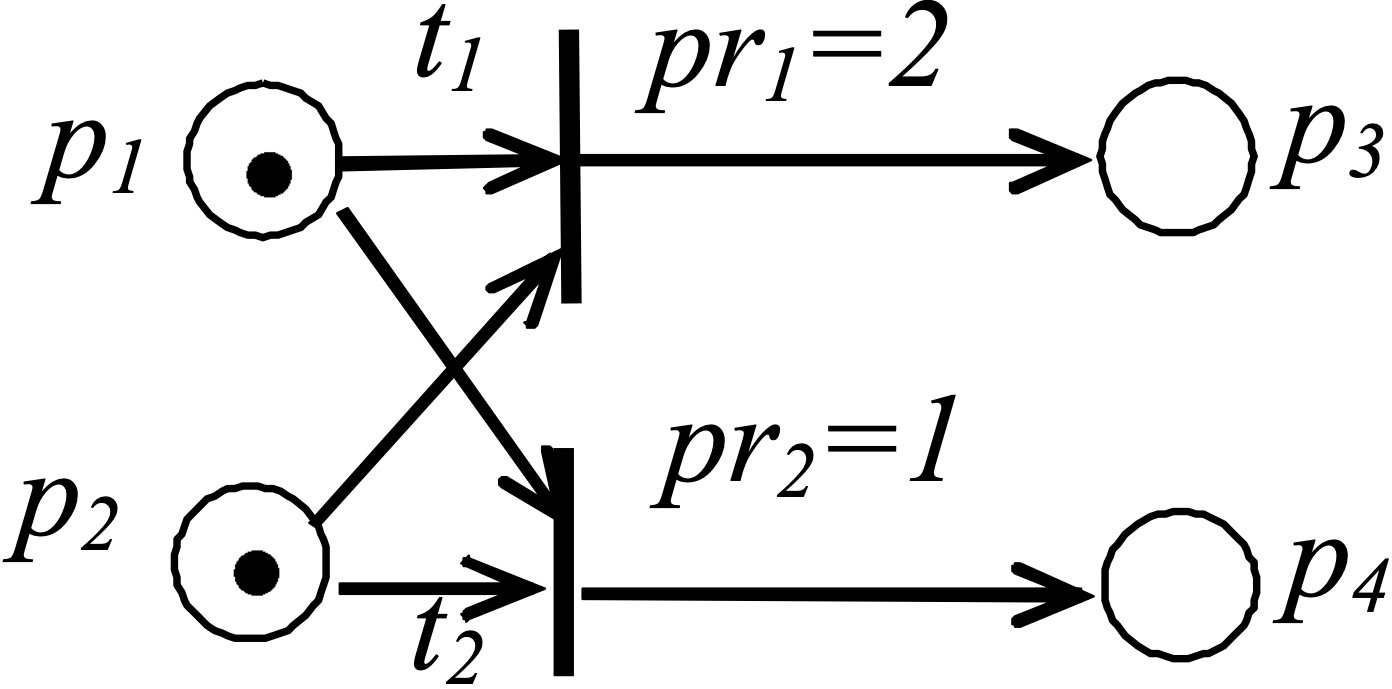
\includegraphics[width=\textwidth]{13/inc/pr1}
        \caption{}
        \label{img:13/inc/pr1}
    \end{subfigure}
    \hspace{.5cm}
    \begin{subfigure}{0.45\textwidth}
        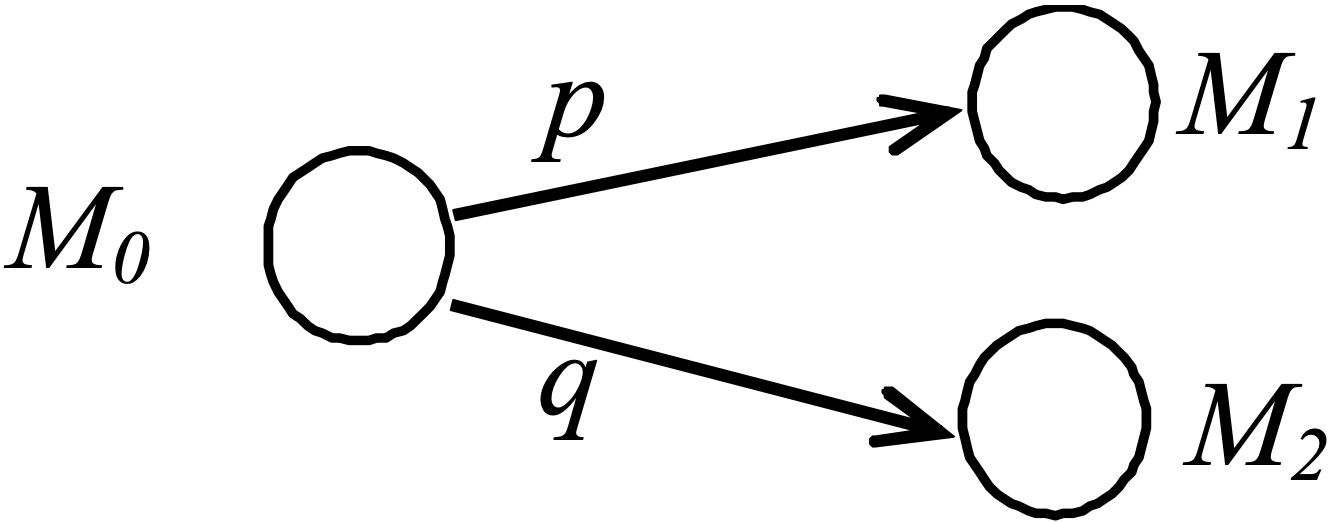
\includegraphics[width=\textwidth]{13/inc/pr2}
        \caption{}
        \label{img:13/inc/pr2}
    \end{subfigure}
    \caption{Пример сети с приоритетами}
\end{figure}

\subsubsection{Сети со случайными срабатываниями переходов}

В описанной выше ситуации, когда имеется возможность срабатывания нескольких переходов ${t_i, t_j, \dots, t_s}$, их приоритет можно задавать вероятностями срабатывания каждого их переходов ${p_i, p_j, \dots, p_s}$, причем ${p_i + p_j + \dots + p_s = 1}$. Тогда исходная маркировка $M_0$ приведет на следующих шагах работы сети к набору маркировок ${M_i, M_j, \dots, M_s}$, каждая из которых будет помечена соответствующей вероятностью. Отождествив маркировки с состоянием сети и положив, что вероятности не зависят от работы сети в предыдущие такты, мы получим цепь Маркова, описывающую вероятностное поведение системы.

Пусть на рисунке~\ref{img:13/inc/pr1} вероятность срабатывания перехода $t_1$ равна $p$, а вероятность срабатывания $t_2$ равна ${q = 1 - p}$. Тогда, обозначив маркировки ${M_0 = [1100]}$, ${M_1 = [0010]}$, ${M_2 = [0001]}$, получим цепь Маркова (рисунок~\ref{img:13/inc/pr2}).

\subsubsection{Иерархические сети} 

Иерархические сети Петри представляют собой многоуровневые структуры, в которых выделяются сети различного уровня. Они позволяют моделировать различные многоуровневые (иерархические) системы.

В отличие от обыкновенных сетей Петри, в иерархических сетях имеются два типа переходов: \textit{простые} и \textit{составные}. Простые переходы ничем не отличаются от рассмотренных ранее, а составные переходы содержат внутри себя сеть Петри более низкого уровня. Формально они состоят из входного (<<головного>>) и выходного (<<хвостового>>) переходов, между ними находится некоторая сеть Петри, которая, в свою очередь, также может быть иерархической.

Пример иерархической сети $N$, в которой имеется составной переход $t_2$, содержащий внутри себя сеть $N'$, показан на рисунке~\ref{img:13/inc/hierarchial}. Составной переход $t_2$ имеет <<голову>> $t_2'$ и <<хвост>> $t_2''$, между которыми заключена сеть $N'$, состоящая из позиций $p_{21}$--$p_{25}$ и переходов $t_{21}$--$t_{23}$. 

\image
{.75\textwidth}
{13/inc/hierarchial}
{Пример иерархической сети Петри}

Иерархическая сеть функционирует, как и обыкновенная СП, переходя от одной маркировки к другой и обмениваясь фишками (в том числе между сетями различного уровня). Исключение составляют правила работы составных переходов.

Срабатывание составных переходов является не мгновенным событием, как в обыкновенных СП, а составным действием. Поэтому говорят не о срабатывании составного перехода, а о его работе. На каждом шаге дискретного времени $\theta$ составной переход может находиться в одном из двух состояний~--- пассивном и активном. Начальное состояние всех переходов~--- пассивное. Составной переход может быть активирован в момент времени $\theta$, если он до этого был пассивен, и имеются условия для срабатывания его головного перехода. При этом производится изменение маркировки в сети верхнего уровня по обычным правилам~(\ref{eq:rule}), и одновременно запускается работа в сети, находящейся внутри составного перехода. Во время ее работы функционирование сети верхнего уровня блокируется. Сеть нижнего уровня работает с учетом своей начальной маркировки до тех пор, пока все ее переходы не станут пассивными (то есть не смогут сработать). После этого происходит срабатывание хвостового перехода и изменение маркировки сети верхнего уровня согласно~(\ref{eq:rule}). Составной переход возвращается в пассивное состояние, а в сети нижнего уровня восстанавливается начальная маркировка.

Ниже приведено дерево маркировок сетей $N$ и $N'$ при указанных на рисунке~\ref{img:13/inc/hierarchial} начальных маркировках.

Мы видим, что на шаге ${\theta = 2}$ происходит работа составного перехода $t_2$ и сети $N'$ в следующем порядке: срабатывание $t_2'$ $\rightarrow$ запуск $N'$ $\rightarrow$ окончание работы $N'$ и восстановление ее начальной маркировки $\rightarrow$ срабатывание $t_2$ и продолжение работы сети $N$.

Отметим также, что описанный процесс напоминает выполнение подпрограммы при программировании на алгоритмических языках. Срабатывание перехода $t_2'$ и соответствует вызову подпрограммы, а срабатывание $t_2''$~--- возврату в основную программу.

\image
{.75\textwidth}
{13/inc/flow}
{}

\subsubsection{Раскрашенные (цветные) сети Петри} 

Раскрашенные сети Петри (РСП, CPN~--- Coloured Petri Net). В ряде приложений перемещаемые в сети Петри ресурсы (фишки) требуется дифференцировать, и тогда
приходится вводить фишки различных видов (например, разных цветов). В этом случае для каждого перехода необходимо указывать, при каких комбинациях фишек во входных позициях он может сработать, и какое количество фишек различных цветов помещается в выходные позиции.

Понятно, что моделирующая возможность раскрашенных сетей Петри выше, чем у обычных, однако при этом значительно усложняется их описание.

Следует отметить, что раскрашенные сети Петри могут быть преобразованы в обычные, но при этом возрастают размеры сети.

Упомянем еще некоторые расширения сетей Петри: синхронные, самомодифицируемые (с изменяющейся кратностью дуг, когда $F^p$ и $F^t$ зависят от $\tau$), и другие.